\documentclass{report}
\renewcommand{\bibname}{Referencias}
\renewcommand\contentsname{\'Indice de Conten\'ido}
\usepackage{graphicx}
\graphicspath{{img/}}
\usepackage{caption}
\usepackage{subcaption}
\usepackage{float}
\usepackage[spanish]{babel}
\usepackage[style=ieee]{biblatex}
\addbibresource{TC_TPF_Director.bib}

\title{\textsc{Director}\\Teoría de la Computación}
\author{Ulises C. Ramirez [ulir19@gmail.com, ulisescolrez@gmail.com]\\Héctor J.
Chripczuk [hectorejch@gmail.com]}
\date{01 de Noviembre, 2018}
\begin{document}
\maketitle
\pagenumbering{gobble}
\newpage
\section*{Versionado}
Para el corriente documento se est\'a llevando un versionado a fin de mantener
un respaldo del trabajo y adem\'as proveer a la c\'atedra o a cualquier
interesado la posibilidad de leer el material en la \'ultima versi\'on disponible.\\

\begin{center}
  \textsc{Repositorio}: \textit{https://github.com/ulisescolina/UC-TC}
\end{center}

\hfill--\textsc{Equipo Director}
\tableofcontents
\pagenumbering{gobble}
\newpage

% === Inicio del Cuerpo del Documento === %
\pagenumbering{arabic}

% Compilado para la seccion que presenta un poco de la investigacion que
% soporta el desarrollo de una herramienta como Director
\section{Método}
\label{sec:metodo}
Al igual que los atributos, los metodos, son componentes dentro del diagrama de
clases que ayudan a la manipulación de los datos, estos brindan el
comportamiento que es propio al objeto. El lenguaje presentado permite definir
métodos de la siguiente manera:

\begin{lstlisting}[caption={BNF - Método}, basicstyle=\footnotesize\ttfamily]
  <metodo>::=<visibilidad><nombre>"("<parametro>")" ":"<tipo>
  <metodo>::=<visibilidad><nombre>"("<parametros>")" ":"<tipo>
\end{lstlisting}

En donde se puede decir que \texttt{parametro(s)} se define de la siguiente
manera:

\begin{lstlisting}[basicstyle=\footnotesize\ttfamily]
  <parametro> ::= <nombre> ":" <tipo>
\end{lstlisting}

\begin{lstlisting}[basicstyle=\footnotesize\ttfamily]
  <parametros> ::= <parametro> | <parametros>
\end{lstlisting}

Director, está dotado de la capacidad para tratar los casos triviales del
manejo de los datos dentro de un objeto, estos casos triviales corresponden a
situaciones en las cuales una de las necesidades de comportammiento para un
objeto viene dado por la urgencia de agregar algún mecanismo que permita
acceder a los atributos del mismo, las acciones comunes de acceso a estos
atributos son las siguientes: definir el valor de un atributo y obtener el
valor de ese atributo, las cuales son solucionadas con los \texttt{setters}
y los \texttt{getters}.

Director, no requiere que se definan explicitamente estos métodos, éste los
genera de manera automática.

Teniendo en cuenta el ejemplo mencionado en la \texttt{Seccion
\ref{sec:atributo}}, Director automáticamente generaría los siguientes métodos
para el lenguaje Java:

\begin{lstlisting}[language=Java, basicstyle=\footnotesize\ttfamily,
label=lst:drt_java_metodo, caption={Java - Generación \texttt{Fragmento \ref{sec:atributo}}}]
  ...
	public String get_nombre(){
		return this.nombre;
		}

	public void set_nombre(String nombre){
		this.nombre = nombre;
		}

	public String get_apellido(){
		return this.apellido;
		}

	public void set_apellido(String apellido){
		this.apellido = apellido;
		}

	public String get_DNI(){
		return this.DNI;
		}

	public void set_DNI(String DNI){
		this.DNI = DNI;
		}
	...
\end{lstlisting}

De todos modos, es posible indicar otros metodos que se deseen incluir en el
modelo. Si agregaramos algun $metodo\_generico$ al ejemplo con el que se viene
trabajando, la lista de atributos y modelos quedaría definida de la siguiente
manera.

\begin{lstlisting}[caption={Director - Declaración de Método}, label=lst:drt_java_modelo_metodo_generico]
	private nombre:string
	private apellido:string
	private DNI:string
	public metodo_generico():void
\end{lstlisting}

Lo que resultaria en la generación del ``esqueleto'' necesario para la
implementación de dicho método. Tomando como base lo que ya se hizo en
el \texttt{Fragmento \ref{lst:drt_java_metodo}}, se le agregaría:

\begin{lstlisting}[caption={Java - Generación metodo\_generico agregado en
\texttt{Fragmento \ref{lst:drt_java_modelo_metodo_generico}}}, language=Java, basicstyle=\footnotesize\ttfamily]
  public void metodo_generico() {
		// Implementacion del metodo
		}
\end{lstlisting}


\subsection*{Autómatas finitos}
\label{sub:metodo_af}

Aquí se proporcionarán los autómatas finitos para la definición de un método y
las subcomponentes que se crearon para éste, como por ejemplo el
\texttt{parametro}.

\begin{figure}[H]
	\centering
	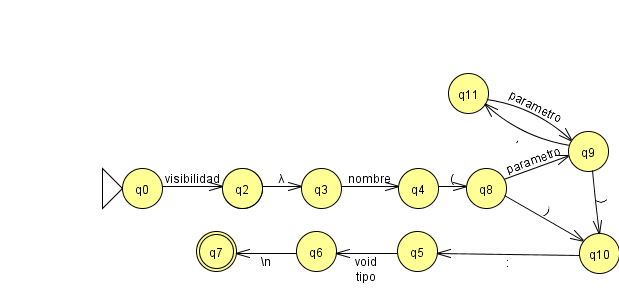
\includegraphics[width=.4\linewidth]{automatas_finitos/metodoDrt.png}
	\caption{Autómata finito - Método}
	\label{fig:metodo_af}
\end{figure}

\begin{figure}[H]
	\centering
	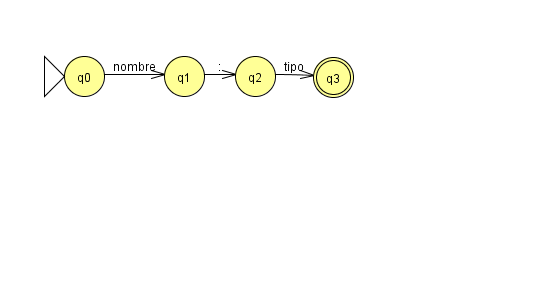
\includegraphics[width=.4\linewidth]{automatas_finitos/parametroDrt.png}
	\caption{Autómata finito - Parámetro}
	\label{fig:metodo_parametro_af}
\end{figure}




\chapter{Problema}
\label{sec:problema}
Descripcion del problema que se pretende mitigar con el lenguaje

% Compilado para la sección dedicada al lenguaje
\section{Método}
\label{sec:metodo}
Al igual que los atributos, los metodos, son componentes dentro del diagrama de
clases que ayudan a la manipulación de los datos, estos brindan el
comportamiento que es propio al objeto. El lenguaje presentado permite definir
métodos de la siguiente manera:

\begin{lstlisting}[caption={BNF - Método}, basicstyle=\footnotesize\ttfamily]
  <metodo>::=<visibilidad><nombre>"("<parametro>")" ":"<tipo>
  <metodo>::=<visibilidad><nombre>"("<parametros>")" ":"<tipo>
\end{lstlisting}

En donde se puede decir que \texttt{parametro(s)} se define de la siguiente
manera:

\begin{lstlisting}[basicstyle=\footnotesize\ttfamily]
  <parametro> ::= <nombre> ":" <tipo>
\end{lstlisting}

\begin{lstlisting}[basicstyle=\footnotesize\ttfamily]
  <parametros> ::= <parametro> | <parametros>
\end{lstlisting}

Director, está dotado de la capacidad para tratar los casos triviales del
manejo de los datos dentro de un objeto, estos casos triviales corresponden a
situaciones en las cuales una de las necesidades de comportammiento para un
objeto viene dado por la urgencia de agregar algún mecanismo que permita
acceder a los atributos del mismo, las acciones comunes de acceso a estos
atributos son las siguientes: definir el valor de un atributo y obtener el
valor de ese atributo, las cuales son solucionadas con los \texttt{setters}
y los \texttt{getters}.

Director, no requiere que se definan explicitamente estos métodos, éste los
genera de manera automática.

Teniendo en cuenta el ejemplo mencionado en la \texttt{Seccion
\ref{sec:atributo}}, Director automáticamente generaría los siguientes métodos
para el lenguaje Java:

\begin{lstlisting}[language=Java, basicstyle=\footnotesize\ttfamily,
label=lst:drt_java_metodo, caption={Java - Generación \texttt{Fragmento \ref{sec:atributo}}}]
  ...
	public String get_nombre(){
		return this.nombre;
		}

	public void set_nombre(String nombre){
		this.nombre = nombre;
		}

	public String get_apellido(){
		return this.apellido;
		}

	public void set_apellido(String apellido){
		this.apellido = apellido;
		}

	public String get_DNI(){
		return this.DNI;
		}

	public void set_DNI(String DNI){
		this.DNI = DNI;
		}
	...
\end{lstlisting}

De todos modos, es posible indicar otros metodos que se deseen incluir en el
modelo. Si agregaramos algun $metodo\_generico$ al ejemplo con el que se viene
trabajando, la lista de atributos y modelos quedaría definida de la siguiente
manera.

\begin{lstlisting}[caption={Director - Declaración de Método}, label=lst:drt_java_modelo_metodo_generico]
	private nombre:string
	private apellido:string
	private DNI:string
	public metodo_generico():void
\end{lstlisting}

Lo que resultaria en la generación del ``esqueleto'' necesario para la
implementación de dicho método. Tomando como base lo que ya se hizo en
el \texttt{Fragmento \ref{lst:drt_java_metodo}}, se le agregaría:

\begin{lstlisting}[caption={Java - Generación metodo\_generico agregado en
\texttt{Fragmento \ref{lst:drt_java_modelo_metodo_generico}}}, language=Java, basicstyle=\footnotesize\ttfamily]
  public void metodo_generico() {
		// Implementacion del metodo
		}
\end{lstlisting}


\subsection*{Autómatas finitos}
\label{sub:metodo_af}

Aquí se proporcionarán los autómatas finitos para la definición de un método y
las subcomponentes que se crearon para éste, como por ejemplo el
\texttt{parametro}.

\begin{figure}[H]
	\centering
	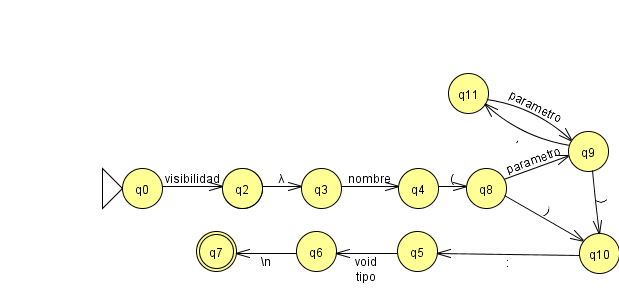
\includegraphics[width=.4\linewidth]{automatas_finitos/metodoDrt.png}
	\caption{Autómata finito - Método}
	\label{fig:metodo_af}
\end{figure}

\begin{figure}[H]
	\centering
	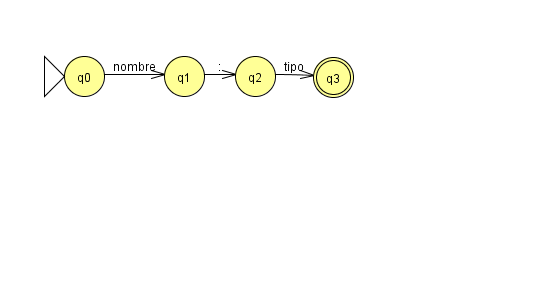
\includegraphics[width=.4\linewidth]{automatas_finitos/parametroDrt.png}
	\caption{Autómata finito - Parámetro}
	\label{fig:metodo_parametro_af}
\end{figure}




% === Bilbiografia === %
\newpage
\printbibliography[title={Referencias}]
\end{document}
